% Options for packages loaded elsewhere
\PassOptionsToPackage{unicode}{hyperref}
\PassOptionsToPackage{hyphens}{url}
\PassOptionsToPackage{dvipsnames,svgnames,x11names}{xcolor}
%
\documentclass[
  letterpaper,
  DIV=11,
  numbers=noendperiod]{scrartcl}

\usepackage{amsmath,amssymb}
\usepackage{lmodern}
\usepackage{iftex}
\ifPDFTeX
  \usepackage[T1]{fontenc}
  \usepackage[utf8]{inputenc}
  \usepackage{textcomp} % provide euro and other symbols
\else % if luatex or xetex
  \usepackage{unicode-math}
  \defaultfontfeatures{Scale=MatchLowercase}
  \defaultfontfeatures[\rmfamily]{Ligatures=TeX,Scale=1}
\fi
% Use upquote if available, for straight quotes in verbatim environments
\IfFileExists{upquote.sty}{\usepackage{upquote}}{}
\IfFileExists{microtype.sty}{% use microtype if available
  \usepackage[]{microtype}
  \UseMicrotypeSet[protrusion]{basicmath} % disable protrusion for tt fonts
}{}
\makeatletter
\@ifundefined{KOMAClassName}{% if non-KOMA class
  \IfFileExists{parskip.sty}{%
    \usepackage{parskip}
  }{% else
    \setlength{\parindent}{0pt}
    \setlength{\parskip}{6pt plus 2pt minus 1pt}}
}{% if KOMA class
  \KOMAoptions{parskip=half}}
\makeatother
\usepackage{xcolor}
\setlength{\emergencystretch}{3em} % prevent overfull lines
\setcounter{secnumdepth}{-\maxdimen} % remove section numbering
% Make \paragraph and \subparagraph free-standing
\ifx\paragraph\undefined\else
  \let\oldparagraph\paragraph
  \renewcommand{\paragraph}[1]{\oldparagraph{#1}\mbox{}}
\fi
\ifx\subparagraph\undefined\else
  \let\oldsubparagraph\subparagraph
  \renewcommand{\subparagraph}[1]{\oldsubparagraph{#1}\mbox{}}
\fi

\usepackage{color}
\usepackage{fancyvrb}
\newcommand{\VerbBar}{|}
\newcommand{\VERB}{\Verb[commandchars=\\\{\}]}
\DefineVerbatimEnvironment{Highlighting}{Verbatim}{commandchars=\\\{\}}
% Add ',fontsize=\small' for more characters per line
\usepackage{framed}
\definecolor{shadecolor}{RGB}{241,243,245}
\newenvironment{Shaded}{\begin{snugshade}}{\end{snugshade}}
\newcommand{\AlertTok}[1]{\textcolor[rgb]{0.68,0.00,0.00}{#1}}
\newcommand{\AnnotationTok}[1]{\textcolor[rgb]{0.37,0.37,0.37}{#1}}
\newcommand{\AttributeTok}[1]{\textcolor[rgb]{0.40,0.45,0.13}{#1}}
\newcommand{\BaseNTok}[1]{\textcolor[rgb]{0.68,0.00,0.00}{#1}}
\newcommand{\BuiltInTok}[1]{\textcolor[rgb]{0.00,0.23,0.31}{#1}}
\newcommand{\CharTok}[1]{\textcolor[rgb]{0.13,0.47,0.30}{#1}}
\newcommand{\CommentTok}[1]{\textcolor[rgb]{0.37,0.37,0.37}{#1}}
\newcommand{\CommentVarTok}[1]{\textcolor[rgb]{0.37,0.37,0.37}{\textit{#1}}}
\newcommand{\ConstantTok}[1]{\textcolor[rgb]{0.56,0.35,0.01}{#1}}
\newcommand{\ControlFlowTok}[1]{\textcolor[rgb]{0.00,0.23,0.31}{#1}}
\newcommand{\DataTypeTok}[1]{\textcolor[rgb]{0.68,0.00,0.00}{#1}}
\newcommand{\DecValTok}[1]{\textcolor[rgb]{0.68,0.00,0.00}{#1}}
\newcommand{\DocumentationTok}[1]{\textcolor[rgb]{0.37,0.37,0.37}{\textit{#1}}}
\newcommand{\ErrorTok}[1]{\textcolor[rgb]{0.68,0.00,0.00}{#1}}
\newcommand{\ExtensionTok}[1]{\textcolor[rgb]{0.00,0.23,0.31}{#1}}
\newcommand{\FloatTok}[1]{\textcolor[rgb]{0.68,0.00,0.00}{#1}}
\newcommand{\FunctionTok}[1]{\textcolor[rgb]{0.28,0.35,0.67}{#1}}
\newcommand{\ImportTok}[1]{\textcolor[rgb]{0.00,0.46,0.62}{#1}}
\newcommand{\InformationTok}[1]{\textcolor[rgb]{0.37,0.37,0.37}{#1}}
\newcommand{\KeywordTok}[1]{\textcolor[rgb]{0.00,0.23,0.31}{#1}}
\newcommand{\NormalTok}[1]{\textcolor[rgb]{0.00,0.23,0.31}{#1}}
\newcommand{\OperatorTok}[1]{\textcolor[rgb]{0.37,0.37,0.37}{#1}}
\newcommand{\OtherTok}[1]{\textcolor[rgb]{0.00,0.23,0.31}{#1}}
\newcommand{\PreprocessorTok}[1]{\textcolor[rgb]{0.68,0.00,0.00}{#1}}
\newcommand{\RegionMarkerTok}[1]{\textcolor[rgb]{0.00,0.23,0.31}{#1}}
\newcommand{\SpecialCharTok}[1]{\textcolor[rgb]{0.37,0.37,0.37}{#1}}
\newcommand{\SpecialStringTok}[1]{\textcolor[rgb]{0.13,0.47,0.30}{#1}}
\newcommand{\StringTok}[1]{\textcolor[rgb]{0.13,0.47,0.30}{#1}}
\newcommand{\VariableTok}[1]{\textcolor[rgb]{0.07,0.07,0.07}{#1}}
\newcommand{\VerbatimStringTok}[1]{\textcolor[rgb]{0.13,0.47,0.30}{#1}}
\newcommand{\WarningTok}[1]{\textcolor[rgb]{0.37,0.37,0.37}{\textit{#1}}}

\providecommand{\tightlist}{%
  \setlength{\itemsep}{0pt}\setlength{\parskip}{0pt}}\usepackage{longtable,booktabs,array}
\usepackage{calc} % for calculating minipage widths
% Correct order of tables after \paragraph or \subparagraph
\usepackage{etoolbox}
\makeatletter
\patchcmd\longtable{\par}{\if@noskipsec\mbox{}\fi\par}{}{}
\makeatother
% Allow footnotes in longtable head/foot
\IfFileExists{footnotehyper.sty}{\usepackage{footnotehyper}}{\usepackage{footnote}}
\makesavenoteenv{longtable}
\usepackage{graphicx}
\makeatletter
\def\maxwidth{\ifdim\Gin@nat@width>\linewidth\linewidth\else\Gin@nat@width\fi}
\def\maxheight{\ifdim\Gin@nat@height>\textheight\textheight\else\Gin@nat@height\fi}
\makeatother
% Scale images if necessary, so that they will not overflow the page
% margins by default, and it is still possible to overwrite the defaults
% using explicit options in \includegraphics[width, height, ...]{}
\setkeys{Gin}{width=\maxwidth,height=\maxheight,keepaspectratio}
% Set default figure placement to htbp
\makeatletter
\def\fps@figure{htbp}
\makeatother

\KOMAoption{captions}{tableheading}
\makeatletter
\makeatother
\makeatletter
\makeatother
\makeatletter
\@ifpackageloaded{caption}{}{\usepackage{caption}}
\AtBeginDocument{%
\ifdefined\contentsname
  \renewcommand*\contentsname{Table of contents}
\else
  \newcommand\contentsname{Table of contents}
\fi
\ifdefined\listfigurename
  \renewcommand*\listfigurename{List of Figures}
\else
  \newcommand\listfigurename{List of Figures}
\fi
\ifdefined\listtablename
  \renewcommand*\listtablename{List of Tables}
\else
  \newcommand\listtablename{List of Tables}
\fi
\ifdefined\figurename
  \renewcommand*\figurename{Figure}
\else
  \newcommand\figurename{Figure}
\fi
\ifdefined\tablename
  \renewcommand*\tablename{Table}
\else
  \newcommand\tablename{Table}
\fi
}
\@ifpackageloaded{float}{}{\usepackage{float}}
\floatstyle{ruled}
\@ifundefined{c@chapter}{\newfloat{codelisting}{h}{lop}}{\newfloat{codelisting}{h}{lop}[chapter]}
\floatname{codelisting}{Listing}
\newcommand*\listoflistings{\listof{codelisting}{List of Listings}}
\makeatother
\makeatletter
\@ifpackageloaded{caption}{}{\usepackage{caption}}
\@ifpackageloaded{subcaption}{}{\usepackage{subcaption}}
\makeatother
\makeatletter
\@ifpackageloaded{tcolorbox}{}{\usepackage[many]{tcolorbox}}
\makeatother
\makeatletter
\@ifundefined{shadecolor}{\definecolor{shadecolor}{rgb}{.97, .97, .97}}
\makeatother
\makeatletter
\makeatother
\ifLuaTeX
  \usepackage{selnolig}  % disable illegal ligatures
\fi
\IfFileExists{bookmark.sty}{\usepackage{bookmark}}{\usepackage{hyperref}}
\IfFileExists{xurl.sty}{\usepackage{xurl}}{} % add URL line breaks if available
\urlstyle{same} % disable monospaced font for URLs
\hypersetup{
  colorlinks=true,
  linkcolor={blue},
  filecolor={Maroon},
  citecolor={Blue},
  urlcolor={Blue},
  pdfcreator={LaTeX via pandoc}}

\author{}
\date{}

\begin{document}
\ifdefined\Shaded\renewenvironment{Shaded}{\begin{tcolorbox}[boxrule=0pt, frame hidden, interior hidden, sharp corners, borderline west={3pt}{0pt}{shadecolor}, enhanced, breakable]}{\end{tcolorbox}}\fi

\begin{Shaded}
\begin{Highlighting}[]
\ImportTok{import}\NormalTok{ pandas }\ImportTok{as}\NormalTok{ pd}
\ImportTok{import}\NormalTok{ numpy }\ImportTok{as}\NormalTok{ np}
\ImportTok{from}\NormalTok{ sklearn.feature\_extraction.text }\ImportTok{import}\NormalTok{ CountVectorizer, TfidfVectorizer}
\ImportTok{from}\NormalTok{ sklearn.metrics }\ImportTok{import}\NormalTok{ confusion\_matrix}
\ImportTok{from}\NormalTok{ sklearn.metrics }\ImportTok{import}\NormalTok{ classification\_report, accuracy\_score}
\ImportTok{import}\NormalTok{ matplotlib.pyplot }\ImportTok{as}\NormalTok{ plt}
\ImportTok{from}\NormalTok{ sklearn.tree }\ImportTok{import}\NormalTok{ plot\_tree}
\ImportTok{from}\NormalTok{ sklearn.utils }\ImportTok{import}\NormalTok{ resample}

\ImportTok{from}\NormalTok{ sklearn.model\_selection }\ImportTok{import}\NormalTok{ cross\_val\_score}
\ImportTok{from}\NormalTok{ sklearn.model\_selection }\ImportTok{import}\NormalTok{ cross\_val\_predict}
\ImportTok{from}\NormalTok{ sklearn.model\_selection }\ImportTok{import}\NormalTok{ train\_test\_split}
\ImportTok{import}\NormalTok{ seaborn }\ImportTok{as}\NormalTok{ sns}
\ImportTok{from}\NormalTok{ sklearn.tree }\ImportTok{import}\NormalTok{ DecisionTreeClassifier}
\ImportTok{from}\NormalTok{ sklearn }\ImportTok{import}\NormalTok{ metrics}
\ImportTok{from}\NormalTok{ wordcloud }\ImportTok{import}\NormalTok{ WordCloud, STOPWORDS}
\end{Highlighting}
\end{Shaded}

\begin{Shaded}
\begin{Highlighting}[]
\NormalTok{df1 }\OperatorTok{=}\NormalTok{ pd.read\_csv(}\StringTok{\textquotesingle{}Clean\_Twitter\_data.csv\textquotesingle{}}\NormalTok{)}
\NormalTok{df2 }\OperatorTok{=}\NormalTok{ pd.read\_csv(}\StringTok{\textquotesingle{}Clean\_Twitter\_data1.csv\textquotesingle{}}\NormalTok{)}
\end{Highlighting}
\end{Shaded}

\begin{Shaded}
\begin{Highlighting}[]
\CommentTok{\# Merge datasets}

\NormalTok{df }\OperatorTok{=}\NormalTok{ pd.concat([df1, df2], ignore\_index}\OperatorTok{=}\VariableTok{True}\NormalTok{)}
\NormalTok{df}
\end{Highlighting}
\end{Shaded}

\begin{longtable}[]{@{}llllllll@{}}
\toprule()
& label & text & clean\_text & Tweet\_tokenized & Tweet\_without\_stop &
Tweet\_stemmed & Tweet\_lemmatized \\
\midrule()
\endhead
0 & fashiontrends & What\textquotesingle s the outfit tonight?
😏\textbackslash n⁠\textbackslash nStreaming Eve... & Whats the outfit
tonight \textbackslash n\textbackslash nStreaming Everywh... &
{[}\textquotesingle whats\textquotesingle,
\textquotesingle the\textquotesingle,
\textquotesingle outfit\textquotesingle,
\textquotesingle tonight\textquotesingle, \textquotesingle streami... &
{[}\textquotesingle whats\textquotesingle,
\textquotesingle outfit\textquotesingle,
\textquotesingle tonight\textquotesingle,
\textquotesingle streaming\textquotesingle, \textquotesingle e... &
{[}\textquotesingle what\textquotesingle,
\textquotesingle outfit\textquotesingle,
\textquotesingle tonight\textquotesingle,
\textquotesingle stream\textquotesingle, \textquotesingle every... &
{[}\textquotesingle whats\textquotesingle,
\textquotesingle outfit\textquotesingle,
\textquotesingle tonight\textquotesingle,
\textquotesingle streaming\textquotesingle, \textquotesingle e... \\
1 & fashiontrends & FESTIVE FEATHERS - \#fashion \#fashionable \#fash...
& FESTIVE FEATHERS fashion fashionable fashiona... &
{[}\textquotesingle festive\textquotesingle,
\textquotesingle feathers\textquotesingle,
\textquotesingle fashion\textquotesingle, \textquotesingle fashionabl...
& {[}\textquotesingle festive\textquotesingle,
\textquotesingle feathers\textquotesingle,
\textquotesingle fashion\textquotesingle, \textquotesingle fashionabl...
& {[}\textquotesingle festiv\textquotesingle,
\textquotesingle feather\textquotesingle,
\textquotesingle fashion\textquotesingle,
\textquotesingle fashion\textquotesingle, \textquotesingle f... &
{[}\textquotesingle festive\textquotesingle,
\textquotesingle feather\textquotesingle,
\textquotesingle fashion\textquotesingle,
\textquotesingle fashionable... \\
2 & fashiontrends & Our classic cloud slides are the comfiest shoe... &
Our classic cloud slides are the comfiest shoe... &
{[}\textquotesingle our\textquotesingle,
\textquotesingle classic\textquotesingle,
\textquotesingle cloud\textquotesingle,
\textquotesingle slides\textquotesingle,
\textquotesingle are\textquotesingle, \textquotesingle... &
{[}\textquotesingle classic\textquotesingle,
\textquotesingle cloud\textquotesingle,
\textquotesingle slides\textquotesingle,
\textquotesingle comfiest\textquotesingle, \textquotesingle sh... &
{[}\textquotesingle classic\textquotesingle,
\textquotesingle cloud\textquotesingle,
\textquotesingle slide\textquotesingle,
\textquotesingle comfiest\textquotesingle, \textquotesingle sho... &
{[}\textquotesingle classic\textquotesingle,
\textquotesingle cloud\textquotesingle,
\textquotesingle slide\textquotesingle,
\textquotesingle comfiest\textquotesingle, \textquotesingle sho... \\
3 & fashiontrends & Trendiest Knitwear At Net-A-Porter \#fashiontre... &
Trendiest Knitwear At NetAPorter fashiontrends... &
{[}\textquotesingle trendiest\textquotesingle,
\textquotesingle knitwear\textquotesingle,
\textquotesingle at\textquotesingle,
\textquotesingle netaporter\textquotesingle, ... &
{[}\textquotesingle trendiest\textquotesingle,
\textquotesingle knitwear\textquotesingle,
\textquotesingle netaporter\textquotesingle, \textquotesingle fashi... &
{[}\textquotesingle trendiest\textquotesingle,
\textquotesingle knitwear\textquotesingle,
\textquotesingle netaport\textquotesingle, \textquotesingle fashion... &
{[}\textquotesingle trendiest\textquotesingle,
\textquotesingle knitwear\textquotesingle,
\textquotesingle netaporter\textquotesingle,
\textquotesingle fashi... \\
4 & fashiontrends & Or like \#Celio, a cool, fun-loving and smart o... &
Or like Celio a cool funloving and smart one\textbackslash n... &
{[}\textquotesingle or\textquotesingle,
\textquotesingle like\textquotesingle,
\textquotesingle celio\textquotesingle,
\textquotesingle a\textquotesingle,
\textquotesingle cool\textquotesingle, \textquotesingle funlovin... &
{[}\textquotesingle like\textquotesingle,
\textquotesingle celio\textquotesingle,
\textquotesingle cool\textquotesingle,
\textquotesingle funloving\textquotesingle,
\textquotesingle smart\textquotesingle... &
{[}\textquotesingle like\textquotesingle,
\textquotesingle celio\textquotesingle,
\textquotesingle cool\textquotesingle,
\textquotesingle funlov\textquotesingle,
\textquotesingle smart\textquotesingle, \textquotesingle... &
{[}\textquotesingle like\textquotesingle,
\textquotesingle celio\textquotesingle,
\textquotesingle cool\textquotesingle,
\textquotesingle funloving\textquotesingle,
\textquotesingle smart\textquotesingle... \\
... & ... & ... & ... & ... & ... & ... & ... \\
197 & ecommerce & ChocoMars - Multi-Purpose WordPress
Theme\textbackslash n\textbackslash n\textbackslash... & ChocoMars
MultiPurpose WordPress
Theme\textbackslash n\textbackslash n\textbackslash nb... &
{[}\textquotesingle chocomars\textquotesingle,
\textquotesingle multipurpose\textquotesingle,
\textquotesingle wordpress\textquotesingle, \textquotesingle th... &
{[}\textquotesingle chocomars\textquotesingle,
\textquotesingle multipurpose\textquotesingle,
\textquotesingle wordpress\textquotesingle, \textquotesingle th... &
{[}\textquotesingle chocomar\textquotesingle,
\textquotesingle multipurpos\textquotesingle,
\textquotesingle wordpress\textquotesingle, \textquotesingle them... &
{[}\textquotesingle chocomars\textquotesingle,
\textquotesingle multipurpose\textquotesingle,
\textquotesingle wordpress\textquotesingle, \textquotesingle th... \\
198 & ecommerce & is for Sale!\textbackslash n\#domain \#domainname
\#domainname... & is for Sale\textbackslash ndomain domainname
domainnamefors... & {[}\textquotesingle\textquotesingle,
\textquotesingle is\textquotesingle,
\textquotesingle for\textquotesingle,
\textquotesingle sale\textquotesingle,
\textquotesingle domain\textquotesingle, \textquotesingle domainnam... &
{[}\textquotesingle\textquotesingle,
\textquotesingle sale\textquotesingle,
\textquotesingle domain\textquotesingle,
\textquotesingle domainname\textquotesingle,
\textquotesingle domainna... & {[}\textquotesingle\textquotesingle,
\textquotesingle sale\textquotesingle,
\textquotesingle domain\textquotesingle,
\textquotesingle domainnam\textquotesingle,
\textquotesingle domainnam... & {[}\textquotesingle\textquotesingle,
\textquotesingle sale\textquotesingle,
\textquotesingle domain\textquotesingle,
\textquotesingle domainname\textquotesingle,
\textquotesingle domainna... \\
199 & ecommerce & WooCommerce Membership
*\textbackslash n\textbackslash n\textbackslash n\#codecanyon \#eco... &
WooCommerce Membership
\textbackslash n\textbackslash n\textbackslash ncodecanyon ecomme... &
{[}\textquotesingle woocommerce\textquotesingle,
\textquotesingle membership\textquotesingle,
\textquotesingle codecanyon\textquotesingle, \textquotesingle e... &
{[}\textquotesingle woocommerce\textquotesingle,
\textquotesingle membership\textquotesingle,
\textquotesingle codecanyon\textquotesingle, \textquotesingle e... &
{[}\textquotesingle woocommerc\textquotesingle,
\textquotesingle membership\textquotesingle,
\textquotesingle codecanyon\textquotesingle, \textquotesingle ec... &
{[}\textquotesingle woocommerce\textquotesingle,
\textquotesingle membership\textquotesingle,
\textquotesingle codecanyon\textquotesingle, \textquotesingle e... \\
200 & ecommerce & How to Create an Omnichannel Fraud Prevention ... &
How to Create an Omnichannel Fraud Prevention ... &
{[}\textquotesingle how\textquotesingle,
\textquotesingle to\textquotesingle,
\textquotesingle create\textquotesingle,
\textquotesingle an\textquotesingle,
\textquotesingle omnichannel\textquotesingle, \textquotesingle... &
{[}\textquotesingle create\textquotesingle,
\textquotesingle omnichannel\textquotesingle,
\textquotesingle fraud\textquotesingle, \textquotesingle prevention... &
{[}\textquotesingle creat\textquotesingle,
\textquotesingle omnichannel\textquotesingle,
\textquotesingle fraud\textquotesingle,
\textquotesingle prevent\textquotesingle, \textquotesingle... &
{[}\textquotesingle create\textquotesingle,
\textquotesingle omnichannel\textquotesingle,
\textquotesingle fraud\textquotesingle,
\textquotesingle prevention... \\
201 & ecommerce & Digita - WooCommerce Parallax
Theme\textbackslash n\textbackslash n\textbackslash n\#comp... & Digita
WooCommerce Parallax
Theme\textbackslash n\textbackslash n\textbackslash ncomput... &
{[}\textquotesingle digita\textquotesingle,
\textquotesingle woocommerce\textquotesingle,
\textquotesingle parallax\textquotesingle,
\textquotesingle theme\textquotesingle,... &
{[}\textquotesingle digita\textquotesingle,
\textquotesingle woocommerce\textquotesingle,
\textquotesingle parallax\textquotesingle,
\textquotesingle theme\textquotesingle,... &
{[}\textquotesingle digita\textquotesingle,
\textquotesingle woocommerc\textquotesingle,
\textquotesingle parallax\textquotesingle,
\textquotesingle theme\textquotesingle, ... &
{[}\textquotesingle digita\textquotesingle,
\textquotesingle woocommerce\textquotesingle,
\textquotesingle parallax\textquotesingle,
\textquotesingle theme\textquotesingle,... \\
\bottomrule()
\end{longtable}

\begin{Shaded}
\begin{Highlighting}[]
\NormalTok{df }\OperatorTok{=}\NormalTok{ df[[}\StringTok{\textquotesingle{}label\textquotesingle{}}\NormalTok{,}\StringTok{\textquotesingle{}Tweet\_lemmatized\textquotesingle{}}\NormalTok{]]}
\NormalTok{df.head()}
\end{Highlighting}
\end{Shaded}

\begin{longtable}[]{@{}lll@{}}
\toprule()
& label & Tweet\_lemmatized \\
\midrule()
\endhead
0 & fashiontrends & {[}\textquotesingle whats\textquotesingle,
\textquotesingle outfit\textquotesingle,
\textquotesingle tonight\textquotesingle,
\textquotesingle streaming\textquotesingle, \textquotesingle e... \\
1 & fashiontrends & {[}\textquotesingle festive\textquotesingle,
\textquotesingle feather\textquotesingle,
\textquotesingle fashion\textquotesingle,
\textquotesingle fashionable... \\
2 & fashiontrends & {[}\textquotesingle classic\textquotesingle,
\textquotesingle cloud\textquotesingle,
\textquotesingle slide\textquotesingle,
\textquotesingle comfiest\textquotesingle, \textquotesingle sho... \\
3 & fashiontrends & {[}\textquotesingle trendiest\textquotesingle,
\textquotesingle knitwear\textquotesingle,
\textquotesingle netaporter\textquotesingle,
\textquotesingle fashi... \\
4 & fashiontrends & {[}\textquotesingle like\textquotesingle,
\textquotesingle celio\textquotesingle,
\textquotesingle cool\textquotesingle,
\textquotesingle funloving\textquotesingle,
\textquotesingle smart\textquotesingle... \\
\bottomrule()
\end{longtable}

\begin{Shaded}
\begin{Highlighting}[]
\NormalTok{final\_tweets}\OperatorTok{=}\NormalTok{[i.replace(}\StringTok{","}\NormalTok{,}\StringTok{""}\NormalTok{).replace(}\StringTok{"["}\NormalTok{,}\StringTok{""}\NormalTok{).replace(}\StringTok{"]"}\NormalTok{,}\StringTok{""}\NormalTok{).replace(}\StringTok{"\textquotesingle{}"}\NormalTok{,}\StringTok{""}\NormalTok{) }\ControlFlowTok{for}\NormalTok{ i }\KeywordTok{in}\NormalTok{ df[}\StringTok{\textquotesingle{}Tweet\_lemmatized\textquotesingle{}}\NormalTok{]]}
\NormalTok{final\_tweets[}\DecValTok{0}\NormalTok{:}\DecValTok{5}\NormalTok{]}
\end{Highlighting}
\end{Shaded}

\begin{verbatim}
['whats outfit tonight streaming everywhere link bio saturday weekend sexpositive weekendmood deephouse techhouse spotify theeveningafter lifestyle fashiontrends styleblogger fashioninspo fashion style model painting makeup fashionblogger ',
 'festive feather fashion fashionable fashionaddict fashionblogger fashionbloggers fashiongram fashionicon fashioninspo fashionista fashionistas fashionlove fashionlovers fashionpost fashionstyle fashiontrends feather festive insta ',
 'classic cloud slide comfiest shoe around shop kat cloud slide today yoru fave color minimal heel fashionrevolution black fashiontrends summerfashion fashioninspo vintagefashion glamour cloudshoes slipper ',
 'trendiest knitwear netaporter fashiontrends via youtube knitwear sweater netaporter fashiontrends',
 'like celio cool funloving smart one trendy fashiontrends lookatme ']
\end{verbatim}

\begin{Shaded}
\begin{Highlighting}[]
\NormalTok{df[}\StringTok{\textquotesingle{}final\_tweets\textquotesingle{}}\NormalTok{]}\OperatorTok{=}\NormalTok{final\_tweets}
\end{Highlighting}
\end{Shaded}

\begin{verbatim}
/var/folders/q0/hps99sh511n627gdy32s4wlh0000gn/T/ipykernel_52383/3791901592.py:1: SettingWithCopyWarning: 
A value is trying to be set on a copy of a slice from a DataFrame.
Try using .loc[row_indexer,col_indexer] = value instead

See the caveats in the documentation: https://pandas.pydata.org/pandas-docs/stable/user_guide/indexing.html#returning-a-view-versus-a-copy
  df['final_tweets']=final_tweets
\end{verbatim}

\begin{Shaded}
\begin{Highlighting}[]
\NormalTok{df}\OperatorTok{=}\NormalTok{df.drop(}\StringTok{\textquotesingle{}Tweet\_lemmatized\textquotesingle{}}\NormalTok{,axis}\OperatorTok{=}\DecValTok{1}\NormalTok{)}
\NormalTok{df.head()}
\end{Highlighting}
\end{Shaded}

\begin{longtable}[]{@{}lll@{}}
\toprule()
& label & final\_tweets \\
\midrule()
\endhead
0 & fashiontrends & whats outfit tonight streaming everywhere link... \\
1 & fashiontrends & festive feather fashion fashionable fashionadd... \\
2 & fashiontrends & classic cloud slide comfiest shoe around shop ... \\
3 & fashiontrends & trendiest knitwear netaporter fashiontrends vi... \\
4 & fashiontrends & like celio cool funloving smart one trendy fas... \\
\bottomrule()
\end{longtable}

\begin{Shaded}
\begin{Highlighting}[]
\NormalTok{ax }\OperatorTok{=}\NormalTok{ df[}\StringTok{\textquotesingle{}label\textquotesingle{}}\NormalTok{].value\_counts().plot(kind}\OperatorTok{=}\StringTok{\textquotesingle{}bar\textquotesingle{}}\NormalTok{,}
\NormalTok{                                    figsize}\OperatorTok{=}\NormalTok{(}\DecValTok{14}\NormalTok{,}\DecValTok{8}\NormalTok{),}
\NormalTok{                                    title}\OperatorTok{=}\StringTok{"Number for labels"}\NormalTok{)}
\NormalTok{ax.set\_xlabel(}\StringTok{"Labels"}\NormalTok{)}
\NormalTok{ax.set\_ylabel(}\StringTok{"Frequency"}\NormalTok{)}
\end{Highlighting}
\end{Shaded}

\begin{verbatim}
Text(0, 0.5, 'Frequency')
\end{verbatim}

\begin{figure}[H]

{\centering 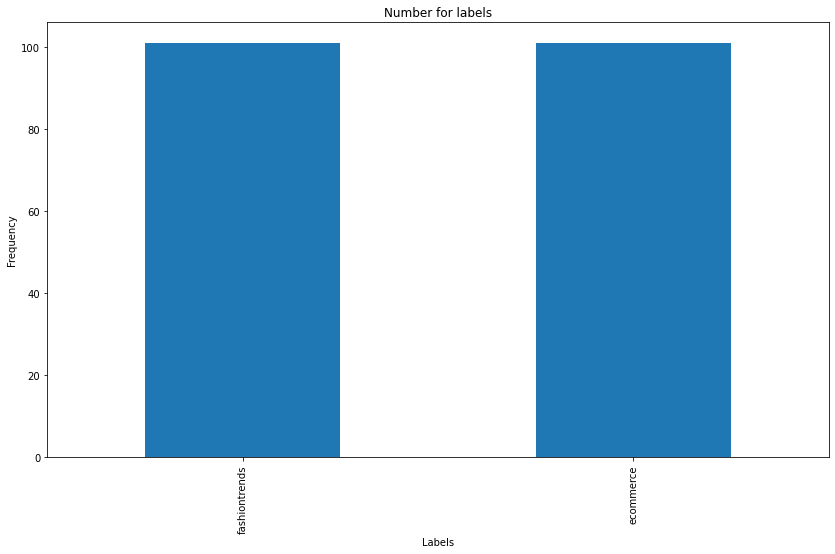
\includegraphics{NBinPy_files/figure-pdf/cell-9-output-2.png}

}

\end{figure}

\begin{Shaded}
\begin{Highlighting}[]
\CommentTok{\# Separate majority and minority classes}

\NormalTok{df\_majority }\OperatorTok{=}\NormalTok{ df[df.label}\OperatorTok{==}\StringTok{\textquotesingle{}fashiontrends\textquotesingle{}}\NormalTok{]}
\NormalTok{df\_minority }\OperatorTok{=}\NormalTok{ df[df.label}\OperatorTok{==}\StringTok{\textquotesingle{}ecommerce\textquotesingle{}}\NormalTok{]}
\end{Highlighting}
\end{Shaded}

\begin{Shaded}
\begin{Highlighting}[]
\CommentTok{\# Downsample majority class}
\NormalTok{df\_majority\_downsampled }\OperatorTok{=}\NormalTok{ resample(df\_majority, }
\NormalTok{                                 replace}\OperatorTok{=}\VariableTok{False}\NormalTok{,    }\CommentTok{\# sample without replacement}
\NormalTok{                                 n\_samples}\OperatorTok{=}\BuiltInTok{len}\NormalTok{(df\_minority),     }\CommentTok{\# to match minority class}
\NormalTok{                                 random\_state}\OperatorTok{=}\DecValTok{123}\NormalTok{) }\CommentTok{\# reproducible results}
 
\CommentTok{\# Combine minority class with downsampled majority class}
\NormalTok{df\_downsampled }\OperatorTok{=}\NormalTok{ pd.concat([df\_majority\_downsampled, df\_minority])}
 
\CommentTok{\# Display new class counts}
\NormalTok{df\_downsampled.label.value\_counts()}
\CommentTok{\# 1    49}
\CommentTok{\# 0    49}
\CommentTok{\# Name: balance, dtype: int64}
\end{Highlighting}
\end{Shaded}

\begin{verbatim}
fashiontrends    101
ecommerce        101
Name: label, dtype: int64
\end{verbatim}

\begin{Shaded}
\begin{Highlighting}[]
\NormalTok{X}\OperatorTok{=}\NormalTok{df\_downsampled[}\StringTok{\textquotesingle{}final\_tweets\textquotesingle{}}\NormalTok{].values}
\NormalTok{y}\OperatorTok{=}\NormalTok{df\_downsampled[}\StringTok{\textquotesingle{}label\textquotesingle{}}\NormalTok{].values}
\end{Highlighting}
\end{Shaded}

\begin{Shaded}
\begin{Highlighting}[]
\ImportTok{from}\NormalTok{ sklearn.preprocessing }\ImportTok{import}\NormalTok{ LabelEncoder}
\NormalTok{labelencoder }\OperatorTok{=}\NormalTok{ LabelEncoder()}
\NormalTok{y }\OperatorTok{=}\NormalTok{ labelencoder.fit\_transform(y)}
\NormalTok{y}
\end{Highlighting}
\end{Shaded}

\begin{verbatim}
array([1, 1, 1, 1, 1, 1, 1, 1, 1, 1, 1, 1, 1, 1, 1, 1, 1, 1, 1, 1, 1, 1,
       1, 1, 1, 1, 1, 1, 1, 1, 1, 1, 1, 1, 1, 1, 1, 1, 1, 1, 1, 1, 1, 1,
       1, 1, 1, 1, 1, 1, 1, 1, 1, 1, 1, 1, 1, 1, 1, 1, 1, 1, 1, 1, 1, 1,
       1, 1, 1, 1, 1, 1, 1, 1, 1, 1, 1, 1, 1, 1, 1, 1, 1, 1, 1, 1, 1, 1,
       1, 1, 1, 1, 1, 1, 1, 1, 1, 1, 1, 1, 1, 0, 0, 0, 0, 0, 0, 0, 0, 0,
       0, 0, 0, 0, 0, 0, 0, 0, 0, 0, 0, 0, 0, 0, 0, 0, 0, 0, 0, 0, 0, 0,
       0, 0, 0, 0, 0, 0, 0, 0, 0, 0, 0, 0, 0, 0, 0, 0, 0, 0, 0, 0, 0, 0,
       0, 0, 0, 0, 0, 0, 0, 0, 0, 0, 0, 0, 0, 0, 0, 0, 0, 0, 0, 0, 0, 0,
       0, 0, 0, 0, 0, 0, 0, 0, 0, 0, 0, 0, 0, 0, 0, 0, 0, 0, 0, 0, 0, 0,
       0, 0, 0, 0])
\end{verbatim}

\begin{Shaded}
\begin{Highlighting}[]
\ImportTok{import}\NormalTok{ random }\ImportTok{as}\NormalTok{ rd}
\NormalTok{MyCV\_content}\OperatorTok{=}\NormalTok{CountVectorizer(}\BuiltInTok{input}\OperatorTok{=}\StringTok{\textquotesingle{}content\textquotesingle{}}\NormalTok{,}
\NormalTok{                        stop\_words}\OperatorTok{=}\StringTok{\textquotesingle{}english\textquotesingle{}}
                        \CommentTok{\#max\_features=100}
\NormalTok{                        )}

\NormalTok{My\_DTM2}\OperatorTok{=}\NormalTok{MyCV\_content.fit\_transform(X)}
\NormalTok{ColNames}\OperatorTok{=}\NormalTok{MyCV\_content.get\_feature\_names()}
\NormalTok{My\_DF\_content}\OperatorTok{=}\NormalTok{pd.DataFrame(My\_DTM2.toarray(),columns}\OperatorTok{=}\NormalTok{ColNames)}


\NormalTok{My\_DF\_content[}\StringTok{\textquotesingle{}LABEL\textquotesingle{}}\NormalTok{] }\OperatorTok{=}\NormalTok{ pd.DataFrame(y,columns}\OperatorTok{=}\NormalTok{[}\StringTok{\textquotesingle{}LABEL\textquotesingle{}}\NormalTok{])}
\NormalTok{rd.seed(}\DecValTok{1993}\NormalTok{)}
\NormalTok{TrainDF, TestDF }\OperatorTok{=}\NormalTok{ train\_test\_split(My\_DF\_content, test\_size}\OperatorTok{=}\FloatTok{0.25}\NormalTok{)}
\NormalTok{TrainLabels}\OperatorTok{=}\NormalTok{TrainDF[}\StringTok{"LABEL"}\NormalTok{]}
\NormalTok{TestLabels}\OperatorTok{=}\NormalTok{TestDF[}\StringTok{"LABEL"}\NormalTok{]}

\NormalTok{TrainDF }\OperatorTok{=}\NormalTok{ TrainDF.drop([}\StringTok{"LABEL"}\NormalTok{], axis}\OperatorTok{=}\DecValTok{1}\NormalTok{)}
\NormalTok{TestDF }\OperatorTok{=}\NormalTok{ TestDF.drop([}\StringTok{"LABEL"}\NormalTok{], axis}\OperatorTok{=}\DecValTok{1}\NormalTok{)}

\ImportTok{from}\NormalTok{ collections }\ImportTok{import}\NormalTok{ Counter}
\NormalTok{Counter(y).keys()}
\NormalTok{Counter(y).values()}
\end{Highlighting}
\end{Shaded}

\begin{verbatim}
/opt/homebrew/Caskroom/miniforge/base/lib/python3.10/site-packages/sklearn/utils/deprecation.py:87: FutureWarning: Function get_feature_names is deprecated; get_feature_names is deprecated in 1.0 and will be removed in 1.2. Please use get_feature_names_out instead.
  warnings.warn(msg, category=FutureWarning)
\end{verbatim}

\begin{verbatim}
dict_values([101, 101])
\end{verbatim}

\begin{Shaded}
\begin{Highlighting}[]
\ImportTok{from}\NormalTok{ sklearn.naive\_bayes }\ImportTok{import}\NormalTok{ MultinomialNB}
\ImportTok{from}\NormalTok{ sklearn }\ImportTok{import}\NormalTok{ metrics}
\ImportTok{from}\NormalTok{ sklearn.metrics }\ImportTok{import}\NormalTok{ confusion\_matrix}

\NormalTok{MyModelNB}\OperatorTok{=}\NormalTok{ MultinomialNB(alpha }\OperatorTok{=} \DecValTok{1}\NormalTok{)}

\NormalTok{NB1}\OperatorTok{=}\NormalTok{MyModelNB.fit(TrainDF, TrainLabels)}
\NormalTok{Preds }\OperatorTok{=}\NormalTok{ MyModelNB.predict(TestDF)}
\NormalTok{Pred\_Proba }\OperatorTok{=}\NormalTok{ MyModelNB.predict\_proba(TestDF)}
\BuiltInTok{print}\NormalTok{(metrics.classification\_report(TestLabels, Preds))}
\NormalTok{cnf\_matrix1 }\OperatorTok{=}\NormalTok{ confusion\_matrix(TestLabels, Preds)}

\CommentTok{\#\#Visualise Confusion Matrix}
\NormalTok{labels }\OperatorTok{=}\NormalTok{ [}\StringTok{\textquotesingle{}fashiontrends\textquotesingle{}}\NormalTok{, }\StringTok{\textquotesingle{}ecommerce\textquotesingle{}}\NormalTok{]}
\NormalTok{ax1}\OperatorTok{=}\NormalTok{plt.subplot()}
\NormalTok{sns.heatmap(confusion\_matrix(TestLabels, Preds), annot}\OperatorTok{=}\VariableTok{True}\NormalTok{, fmt}\OperatorTok{=}\StringTok{\textquotesingle{}g\textquotesingle{}}\NormalTok{, ax}\OperatorTok{=}\NormalTok{ax1)}\OperatorTok{;}

\CommentTok{\# labels, title and ticks}
\NormalTok{ax1.set\_xlabel(}\StringTok{\textquotesingle{}Predicted labels\textquotesingle{}}\NormalTok{)}\OperatorTok{;}\NormalTok{ax1.set\_ylabel(}\StringTok{\textquotesingle{}True labels\textquotesingle{}}\NormalTok{)}\OperatorTok{;} 
\NormalTok{ax1.set\_title(}\StringTok{\textquotesingle{}Confusion Matrix\textquotesingle{}}\NormalTok{)}\OperatorTok{;} 
\NormalTok{ax1.xaxis.set\_ticklabels(labels)}\OperatorTok{;}\NormalTok{ ax1.yaxis.set\_ticklabels(labels)}\OperatorTok{;}
\NormalTok{plt.show()}
\NormalTok{plt.close()}
\end{Highlighting}
\end{Shaded}

\begin{verbatim}
              precision    recall  f1-score   support

           0       0.96      1.00      0.98        25
           1       1.00      0.96      0.98        26

    accuracy                           0.98        51
   macro avg       0.98      0.98      0.98        51
weighted avg       0.98      0.98      0.98        51
\end{verbatim}

\begin{figure}[H]

{\centering 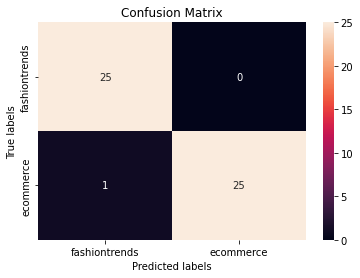
\includegraphics{NBinPy_files/figure-pdf/cell-15-output-2.png}

}

\end{figure}

\begin{Shaded}
\begin{Highlighting}[]
\NormalTok{MyModelNB2}\OperatorTok{=}\NormalTok{ MultinomialNB(alpha }\OperatorTok{=}\DecValTok{3}\NormalTok{)}

\NormalTok{NB2}\OperatorTok{=}\NormalTok{MyModelNB2.fit(TrainDF, TrainLabels)}
\NormalTok{Preds2 }\OperatorTok{=}\NormalTok{ MyModelNB2.predict(TestDF)}
\NormalTok{Pred\_Proba2 }\OperatorTok{=}\NormalTok{ MyModelNB2.predict\_proba(TestDF)}
\BuiltInTok{print}\NormalTok{(metrics.classification\_report(TestLabels, Preds2))}
\NormalTok{cnf\_matrix1 }\OperatorTok{=}\NormalTok{ confusion\_matrix(TestLabels, Preds2)}

\CommentTok{\#\#Visualise Confusion Matrix}
\NormalTok{labels }\OperatorTok{=}\NormalTok{ [}\StringTok{\textquotesingle{}fashiontrends\textquotesingle{}}\NormalTok{, }\StringTok{\textquotesingle{}ecommerce\textquotesingle{}}\NormalTok{]}
\NormalTok{ax1}\OperatorTok{=}\NormalTok{plt.subplot()}
\NormalTok{sns.heatmap(confusion\_matrix(TestLabels, Preds2), annot}\OperatorTok{=}\VariableTok{True}\NormalTok{, fmt}\OperatorTok{=}\StringTok{\textquotesingle{}g\textquotesingle{}}\NormalTok{, ax}\OperatorTok{=}\NormalTok{ax1)}\OperatorTok{;}

\CommentTok{\# labels, title and ticks}
\NormalTok{ax1.set\_xlabel(}\StringTok{\textquotesingle{}Predicted labels\textquotesingle{}}\NormalTok{)}\OperatorTok{;}\NormalTok{ax1.set\_ylabel(}\StringTok{\textquotesingle{}True labels\textquotesingle{}}\NormalTok{)}\OperatorTok{;} 
\NormalTok{ax1.set\_title(}\StringTok{\textquotesingle{}Confusion Matrix\textquotesingle{}}\NormalTok{)}\OperatorTok{;} 
\NormalTok{ax1.xaxis.set\_ticklabels(labels)}\OperatorTok{;}\NormalTok{ ax1.yaxis.set\_ticklabels(labels)}\OperatorTok{;}
\NormalTok{plt.show()}
\NormalTok{plt.close()}
\end{Highlighting}
\end{Shaded}

\begin{verbatim}
              precision    recall  f1-score   support

           0       0.96      1.00      0.98        25
           1       1.00      0.96      0.98        26

    accuracy                           0.98        51
   macro avg       0.98      0.98      0.98        51
weighted avg       0.98      0.98      0.98        51
\end{verbatim}

\begin{figure}[H]

{\centering 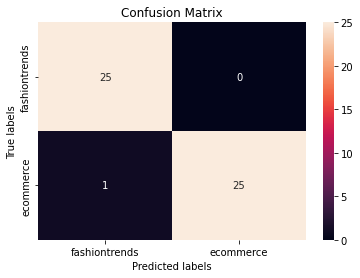
\includegraphics{NBinPy_files/figure-pdf/cell-16-output-2.png}

}

\end{figure}

\begin{Shaded}
\begin{Highlighting}[]
\NormalTok{MyModelNB3}\OperatorTok{=}\NormalTok{ MultinomialNB(alpha }\OperatorTok{=}\DecValTok{0}\NormalTok{)}

\NormalTok{NB3}\OperatorTok{=}\NormalTok{MyModelNB3.fit(TrainDF, TrainLabels)}
\NormalTok{Preds3 }\OperatorTok{=}\NormalTok{ MyModelNB3.predict(TestDF)}
\NormalTok{Pred\_Proba3 }\OperatorTok{=}\NormalTok{ MyModelNB3.predict\_proba(TestDF)}
\BuiltInTok{print}\NormalTok{(metrics.classification\_report(TestLabels, Preds3))}
\NormalTok{cnf\_matrix1 }\OperatorTok{=}\NormalTok{ confusion\_matrix(TestLabels, Preds3)}

\CommentTok{\#\#Visualise Confusion Matrix}
\NormalTok{labels }\OperatorTok{=}\NormalTok{ [}\StringTok{\textquotesingle{}fashiontrennds\textquotesingle{}}\NormalTok{, }\StringTok{\textquotesingle{}ecommerce\textquotesingle{}}\NormalTok{]}
\NormalTok{ax1}\OperatorTok{=}\NormalTok{plt.subplot()}
\NormalTok{sns.heatmap(confusion\_matrix(TestLabels, Preds3), annot}\OperatorTok{=}\VariableTok{True}\NormalTok{, fmt}\OperatorTok{=}\StringTok{\textquotesingle{}g\textquotesingle{}}\NormalTok{, ax}\OperatorTok{=}\NormalTok{ax1)}\OperatorTok{;}

\CommentTok{\# labels, title and ticks}
\NormalTok{ax1.set\_xlabel(}\StringTok{\textquotesingle{}Predicted labels\textquotesingle{}}\NormalTok{)}\OperatorTok{;}\NormalTok{ax1.set\_ylabel(}\StringTok{\textquotesingle{}True labels\textquotesingle{}}\NormalTok{)}\OperatorTok{;} 
\NormalTok{ax1.set\_title(}\StringTok{\textquotesingle{}Confusion Matrix\textquotesingle{}}\NormalTok{)}\OperatorTok{;} 
\NormalTok{ax1.xaxis.set\_ticklabels(labels)}\OperatorTok{;}\NormalTok{ ax1.yaxis.set\_ticklabels(labels)}\OperatorTok{;}
\NormalTok{plt.show()}
\NormalTok{plt.close()}
\end{Highlighting}
\end{Shaded}

\begin{verbatim}
              precision    recall  f1-score   support

           0       0.93      1.00      0.96        25
           1       1.00      0.92      0.96        26

    accuracy                           0.96        51
   macro avg       0.96      0.96      0.96        51
weighted avg       0.96      0.96      0.96        51
\end{verbatim}

\begin{verbatim}
/opt/homebrew/Caskroom/miniforge/base/lib/python3.10/site-packages/sklearn/naive_bayes.py:591: UserWarning: alpha too small will result in numeric errors, setting alpha = 1.0e-10
  warnings.warn(
\end{verbatim}

\begin{figure}[H]

{\centering 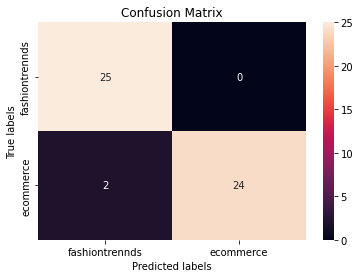
\includegraphics{NBinPy_files/figure-pdf/cell-17-output-3.png}

}

\end{figure}

\begin{Shaded}
\begin{Highlighting}[]
\NormalTok{class\_0\_prob\_sorted }\OperatorTok{=}\NormalTok{ NB1.feature\_log\_prob\_[}\DecValTok{0}\NormalTok{, :].argsort()[::}\OperatorTok{{-}}\DecValTok{1}\NormalTok{]}
\NormalTok{class\_1\_prob\_sorted }\OperatorTok{=}\NormalTok{ NB1.feature\_log\_prob\_[}\DecValTok{1}\NormalTok{, :].argsort()[::}\OperatorTok{{-}}\DecValTok{1}\NormalTok{]}

\BuiltInTok{print}\NormalTok{(np.take(MyCV\_content.get\_feature\_names(), class\_0\_prob\_sorted[:}\DecValTok{10}\NormalTok{]))}
\NormalTok{word\_cloud\_0 }\OperatorTok{=}\NormalTok{ Counter(np.take(MyCV\_content.get\_feature\_names(), class\_0\_prob\_sorted[:}\DecValTok{20}\NormalTok{]))}
\BuiltInTok{print}\NormalTok{(np.take(MyCV\_content.get\_feature\_names(), class\_1\_prob\_sorted[:}\DecValTok{10}\NormalTok{])) }
\NormalTok{word\_cloud\_1 }\OperatorTok{=}\NormalTok{ Counter(np.take(MyCV\_content.get\_feature\_names(), class\_1\_prob\_sorted[:}\DecValTok{20}\NormalTok{]))}
\end{Highlighting}
\end{Shaded}

\begin{verbatim}
['ecommerce' 'business' 'amazon' 'seller' 'addtocart' 'shopify'
 'marketing' 'trending' 'logo' 'retail']
['fashiontrends' 'fashion' 'fashionblogger' 'fashionstyle' 'woman'
 'accessory' 'fashiondesigner' 'clothing' 'fashionaddict' 'holla']
\end{verbatim}

\begin{verbatim}
/opt/homebrew/Caskroom/miniforge/base/lib/python3.10/site-packages/sklearn/utils/deprecation.py:87: FutureWarning: Function get_feature_names is deprecated; get_feature_names is deprecated in 1.0 and will be removed in 1.2. Please use get_feature_names_out instead.
  warnings.warn(msg, category=FutureWarning)
\end{verbatim}

\begin{Shaded}
\begin{Highlighting}[]
\ImportTok{from}\NormalTok{ wordcloud }\ImportTok{import}\NormalTok{ WordCloud, STOPWORDS, ImageColorGenerator}
\NormalTok{wordcloud }\OperatorTok{=}\NormalTok{ WordCloud(background\_color}\OperatorTok{=}\StringTok{\textquotesingle{}white\textquotesingle{}}\NormalTok{).fit\_words(word\_cloud\_0)}

\NormalTok{fig, ax }\OperatorTok{=}\NormalTok{ plt.subplots(figsize}\OperatorTok{=}\NormalTok{(}\DecValTok{15}\NormalTok{,}\DecValTok{15}\NormalTok{))}
\NormalTok{\_ }\OperatorTok{=}\NormalTok{ ax.imshow(wordcloud, interpolation}\OperatorTok{=}\StringTok{\textquotesingle{}bilinear\textquotesingle{}}\NormalTok{)}
\NormalTok{\_ }\OperatorTok{=}\NormalTok{ ax.axis(}\StringTok{"off"}\NormalTok{)}




\NormalTok{wordcloud }\OperatorTok{=}\NormalTok{ WordCloud(background\_color}\OperatorTok{=}\StringTok{\textquotesingle{}white\textquotesingle{}}\NormalTok{).fit\_words(word\_cloud\_1)}

\NormalTok{fig, ax }\OperatorTok{=}\NormalTok{ plt.subplots(figsize}\OperatorTok{=}\NormalTok{(}\DecValTok{15}\NormalTok{,}\DecValTok{15}\NormalTok{))}
\NormalTok{\_ }\OperatorTok{=}\NormalTok{ ax.imshow(wordcloud, interpolation}\OperatorTok{=}\StringTok{\textquotesingle{}bilinear\textquotesingle{}}\NormalTok{)}
\NormalTok{\_ }\OperatorTok{=}\NormalTok{ ax.axis(}\StringTok{"off"}\NormalTok{)}
\end{Highlighting}
\end{Shaded}

\begin{figure}[H]

{\centering 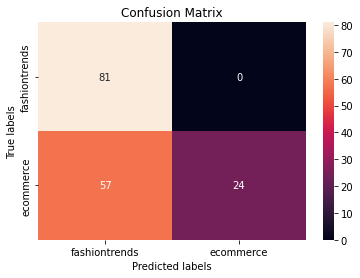
\includegraphics{NBinPy_files/figure-pdf/cell-19-output-1.png}

}

\end{figure}

\begin{figure}[H]

{\centering 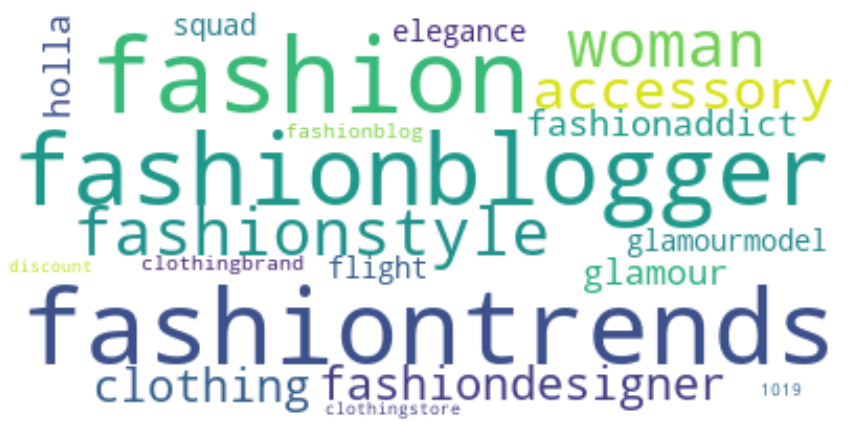
\includegraphics{NBinPy_files/figure-pdf/cell-19-output-2.png}

}

\end{figure}



\end{document}
